\chapter{Experiments}
\label{app:Experiments}

All experiments were ran on an Amazon EC2 t2.micro instances. These
are cloud servers with 1GB of ram and 1 CPU core. These servers
were setup with Ubuntu and the tools needed to run the websites.
Both servers were located in the US (East).

\section{Page Load Speed}
\label{sec:pageLoadSpeeds}

Each page of the website was loaded three times with an average being
given. The result recorded is the time it takes to load all the files
on the web page. This
value is taken from the `Finish' value located at the bottom of
the Chromium developer console in the `Network' tab. These
experiments were done with caching turned off. Times were measured
in milliseconds. The experiments also started with a fresh website,
i.e. no users or messages. For redirects, the HTML values is recorded
for the page that started the redirect.

\begin{table}[H]
	\caption{Home Page load speed}
	\begin{center}
		\begin{tabular}{ | l | l | l |}
			\hline
			Run & Yesod Page & Django Page \\
			1 & 504 & 750 \\
			2 & 512 & 754 \\
			3 & 517 & 756 \\
			Average & 511 & 753.33 \\
			\hline
		\end{tabular}
	\end{center}
	\label{tab:pageLoadSpeeds}
\end{table}

\begin{table}[H]
	\caption{Search Page load speed}
	\begin{center}
		\begin{tabular}{ | l | l | l |}
			\hline
			Run & Yesod Page & Django Page \\
			1 & 541 & 739 \\
			2 & 510 & 768 \\
			3 & 501 & 762 \\
			Average & 517.33 & 756.33 \\
			\hline
		\end{tabular}
	\end{center}
	\label{tab:searchLoadSpeeds}
\end{table}

\begin{table}[H]
	\caption{Login Page load speed}
	\begin{center}
		\begin{tabular}{ | l | l | l |}
			\hline
			Run  & Yesod Page & Django Page \\
			1 & 401 & 767 \\
			2 & 413 & 843 \\
			3 & 517 & 854 \\
			Average & 443.67 & 821.33 \\
			\hline
		\end{tabular}
	\end{center}
	\label{tab:loginLoadSpeeds}
\end{table}

\begin{table}[H]
	\caption{Signup Page load speed}
	\begin{center}
		\begin{tabular}{ | l | l | l |}
			\hline
			Run & Yesod Page & Django Page \\
			1 & 509 & 775 \\
			2 & 479 & 739 \\
			3 & 483 & 778 \\
			Average & 490.33 & 764 \\
			\hline
		\end{tabular}
	\end{center}
	\label{tab:signupLoadSpeeds}
\end{table}

\begin{table}[H]
	\caption{Create an account load speed}
	\begin{center}
		\begin{tabular}{ | l | l | l |}
			\hline
			Run & Yesod Page & Django Page \\
			1 & 510 & 728 \\
			2 & 500 & 751 \\
			3 & 503 & 767 \\
			Average & 504.33 & 748.67 \\
			\hline
		\end{tabular}
	\end{center}
	\label{tab:signupCreateLoadSpeeds}
\end{table}

\begin{table}[H]
	\caption{Log in to an account speed}
	\begin{center}
		\begin{tabular}{ | l | l | l |}
			\hline
			Run & Yesod Page & Django Page \\
			1 & 514 & 643 \\
			2 & 570 & 760 \\
			3 & 558 & 765 \\
			Average & 547.33 & 722.67 \\
			\hline
		\end{tabular}
	\end{center}
	\label{tab:loginLoginLoadSpeeds}
\end{table}

\begin{table}[H]
	\caption{Logout load speed speed}
	\begin{center}
		\begin{tabular}{ | l | | l | l |}
			\hline
			Run & Yesod Page & Django Page \\
			1 & 496 & 770 \\
			2 & 525 & 750 \\
			3 & 510 & 762 \\
			Average & 510.33 & 761.33 \\
			\hline
		\end{tabular}
	\end{center}
	\label{tab:logoutLoadSpeeds}
\end{table}

\begin{table}[H]
	\caption{Current user's profile page}
	\begin{center}
		\begin{tabular}{ | l | | l | l |}
			\hline
			Run & Yesod Page & Django Page \\
			1 & 560 & 931 \\
			2 & 660 & 936 \\
			3 & 631 & 923 \\
			Average & 617 & 930 \\
			\hline
		\end{tabular}
	\end{center}
	\label{tab:currentProfileLoadSpeeds}
\end{table}

\begin{table}[H]
	\caption{Creating message `test'}
	\begin{center}
		\begin{tabular}{ | l | l | l |}
			\hline
			Run & Yesod Page & Django Page \\
			1 & 680 & 811 \\
			2 & 667 & 806 \\
			3 & 691 & 929 \\
			Average & 679.33 & 848.67 \\
			\hline
		\end{tabular}
	\end{center}
	\label{tab:createMessageLoadSpeeds}
\end{table}

\begin{table}[H]
	\caption{Other profile page with three messages}
	\begin{center}
		\begin{tabular}{ | l | l | l |}
			\hline
			Run & Yesod Page & Django Page \\
			1 & 670 & 936 \\
			2 & 643 & 931 \\
			3 & 641 & 859 \\
			Average & 651.33 & 908.67 \\
			\hline
		\end{tabular}
	\end{center}
	\label{tab:otherProfileLoadSpeeds}
\end{table}

\begin{table}[H]
	\caption{Search for message `test', three results}
	\begin{center}
		\begin{tabular}{ | l | l | l |}
			\hline
			Run & Yesod Page & Django Page \\
			1 & 514 & 781 \\
			2 & 502 & 773 \\
			3 & 524 & 745 \\
			Average & 513.33 & 766.33 \\
			\hline
		\end{tabular}
	\end{center}
	\label{tab:searchMessageLoadSpeeds}
\end{table}

\begin{table}[H]
	\caption{Search for user `test', five results}
	\begin{center}
		\begin{tabular}{ | l | l | l |}
			\hline
			Run & Yesod Page & Django Page \\
			1 & 524 & 774 \\
			2 & 516 & 748 \\
			3 & 517 & 748 \\
			Average & 519 & 756.67 \\
			\hline
		\end{tabular}
	\end{center}
	\label{tab:searchUserLoadSpeeds}
\end{table}

\section{Resource Usage}

For Yesod, a Keter bundle is deployed on the server. Keter is a deployment
manager written in Haskell and Yesod has built in support for Keter. On
the Django server, nginx is used, a popular open source web server. On the
server, a Django server is created, and nginx uses the Django server to
deal with incoming requests. All values in this section were acquired
through htop.

On the Yesod server, after running all the tests in the previous section,
total RAM usage was 109MB. Keter's main process and sub-processes used about 
83MB of RAM, with 56MB being shared. The Django
server's RAM usage was at 125MB of RAM, with Django and gunicorn using around
65MB of RAM, sharing 19MB, and nginx using 6MB of RAM, sharing 3MB. This gives
a total of 71MB of RAM being used on the Django server, with 22MB of RAM being
shared. Htop sreenshots are included below.

\begin{figure}[H]
	\centering
	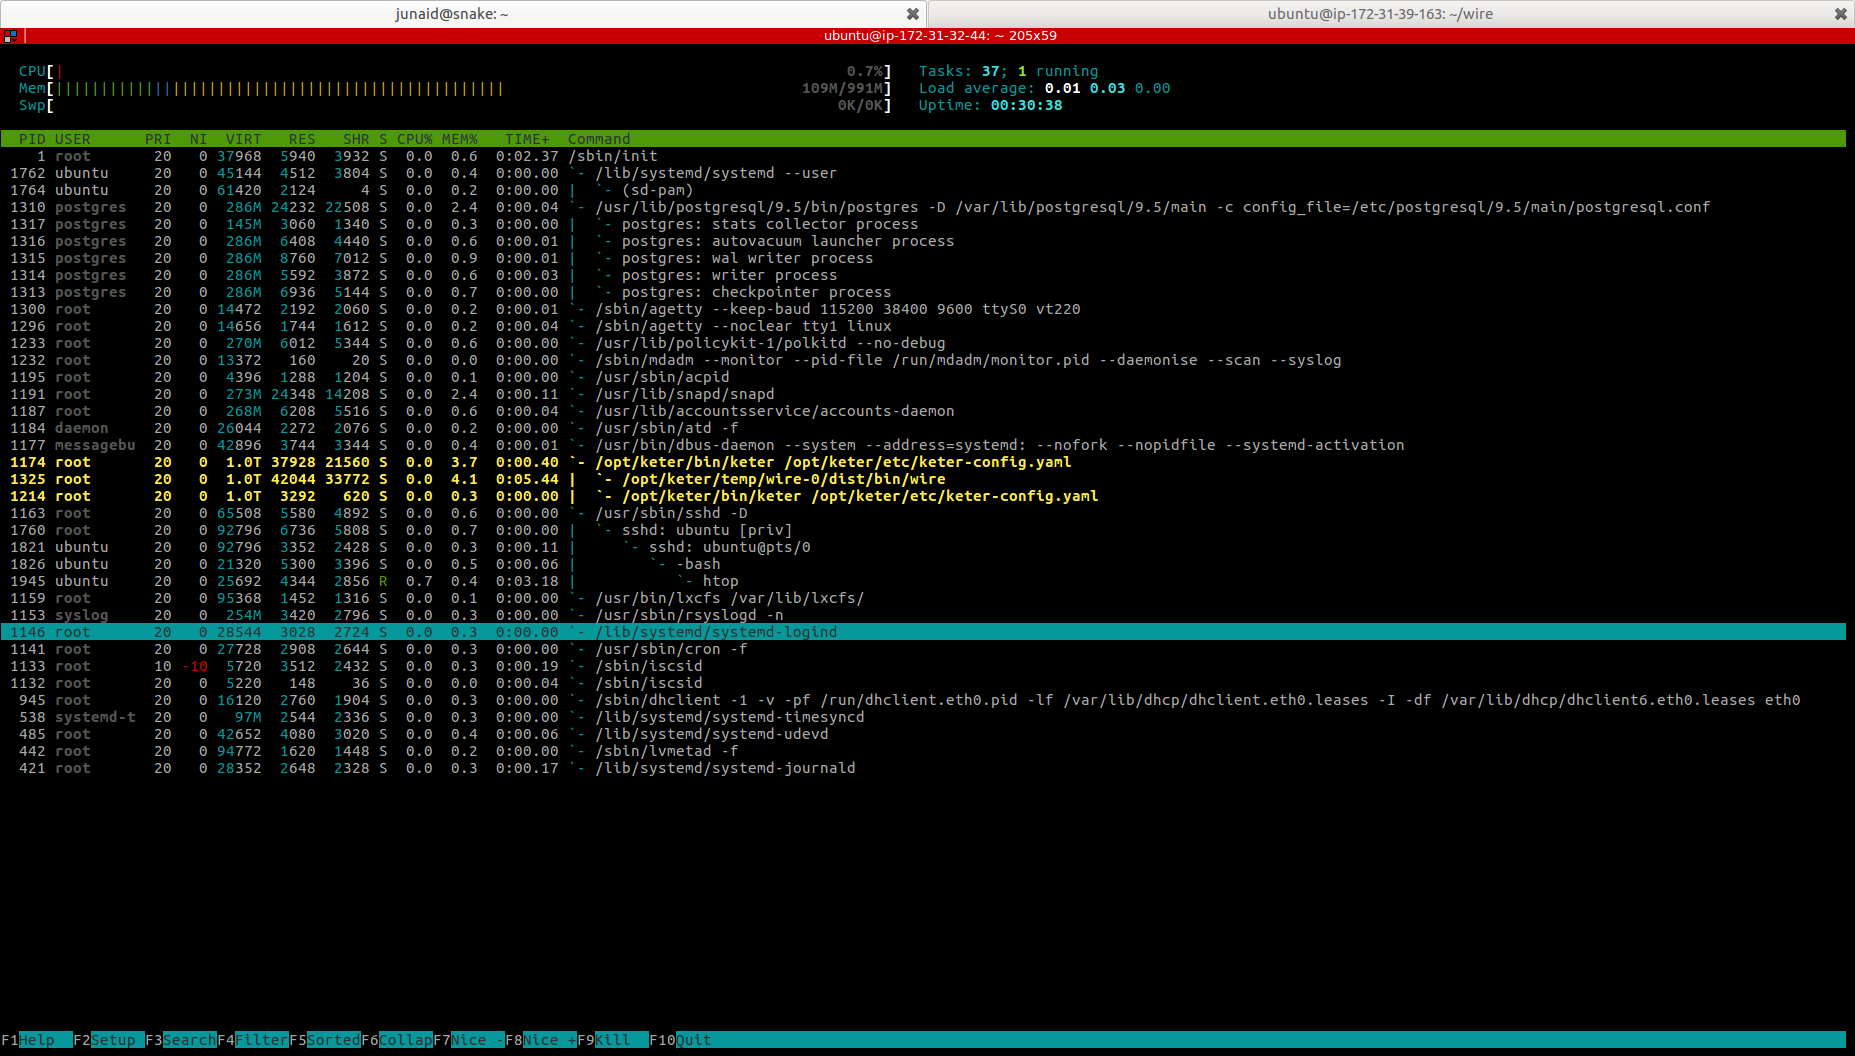
\includegraphics[width=1\textwidth]{final_report/pics/yesodIdle.png}
	\caption{Yesod htop output}
	\label{fig:yesodHtop}
\end{figure}

\begin{figure}[H]
	\centering
	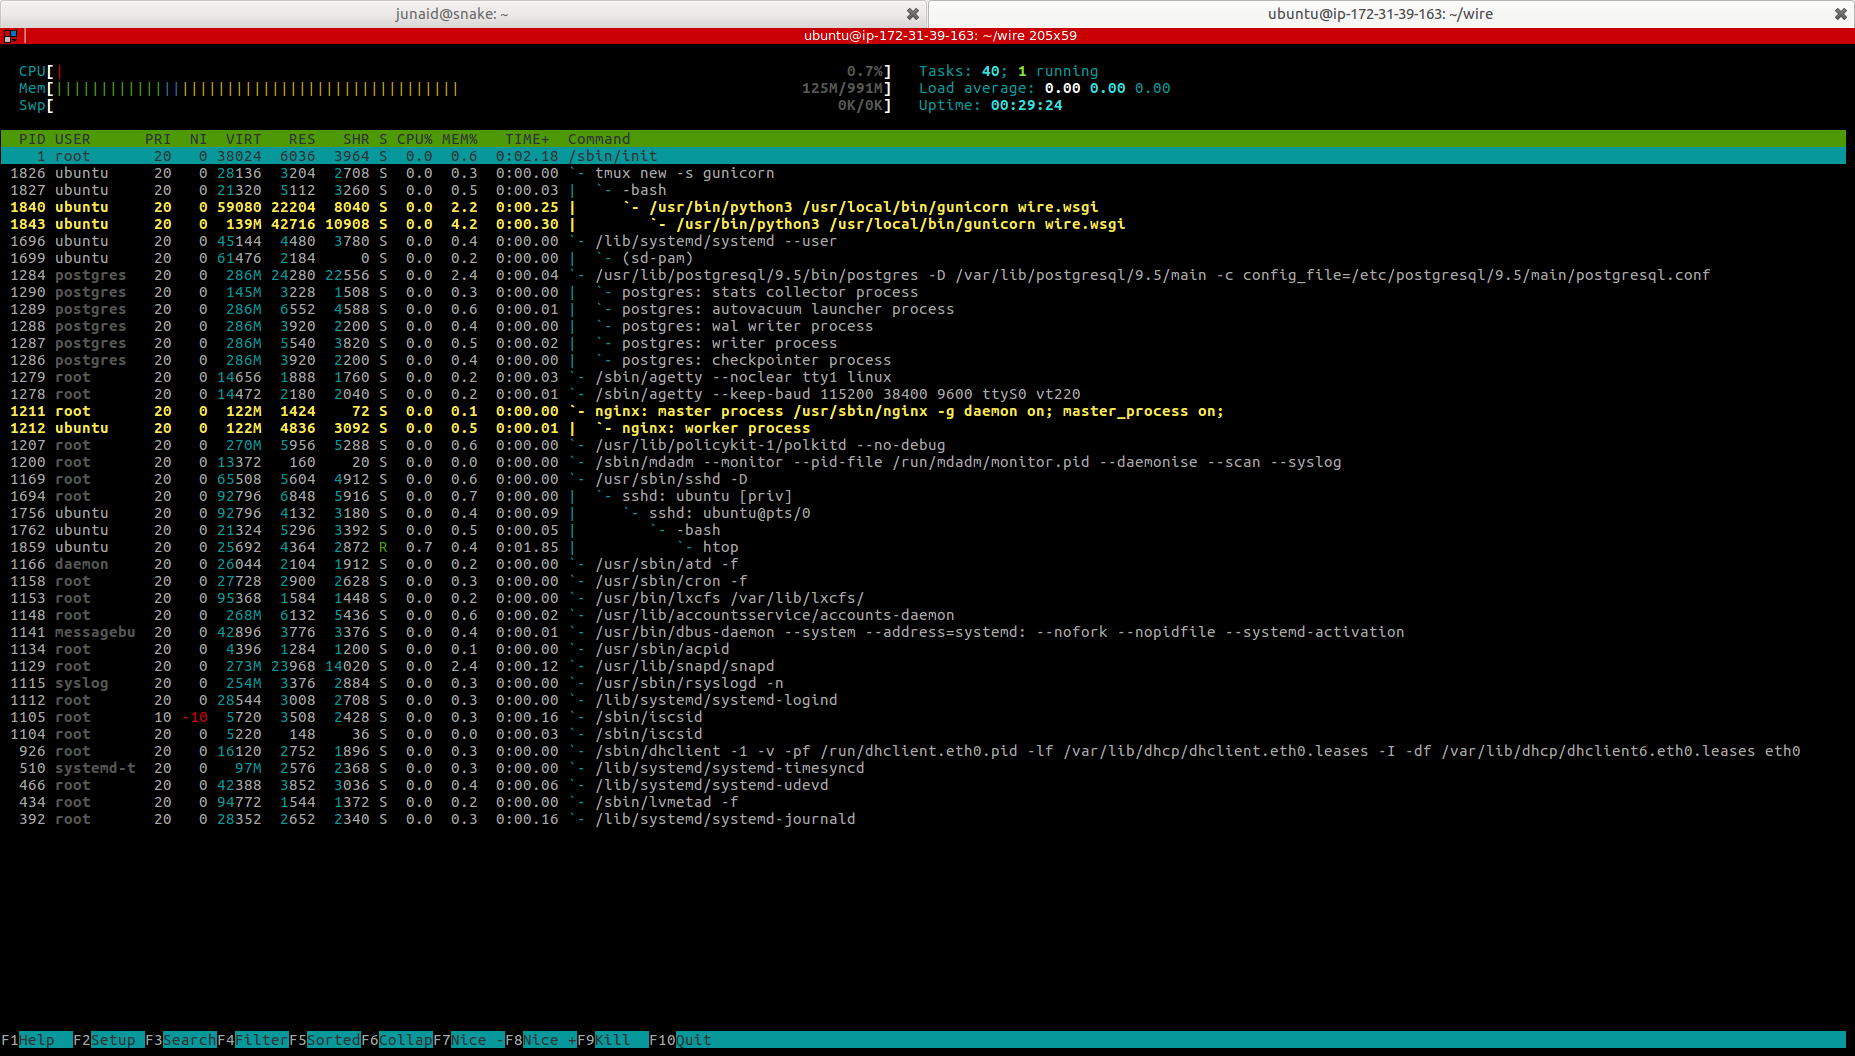
\includegraphics[width=1\textwidth]{final_report/pics/djangoIdle.png}
	\caption{Django htop output}
	\label{fig:djangoHtop}
\end{figure}

\section{Continuous Integration Build Times}

Both frameworks are stored on a git repository on GitHub. Whenever there is a
new commit, Travis CI, a continuous integration tools, starts to build
both frameworks and run tests. The tool will tell you whether or not tests
have passed. Django builds take around 2.5 minutes. Yesod builds take around
3.5-4 minutes. It should be noted that the first Yesod build took 32 minutes.
This was because the first build had to compile all the library files in the
Yesod project. Once these are compiled, they are cached, allowing them to
be used for future builds.

\begin{figure}[H]
	\centering
	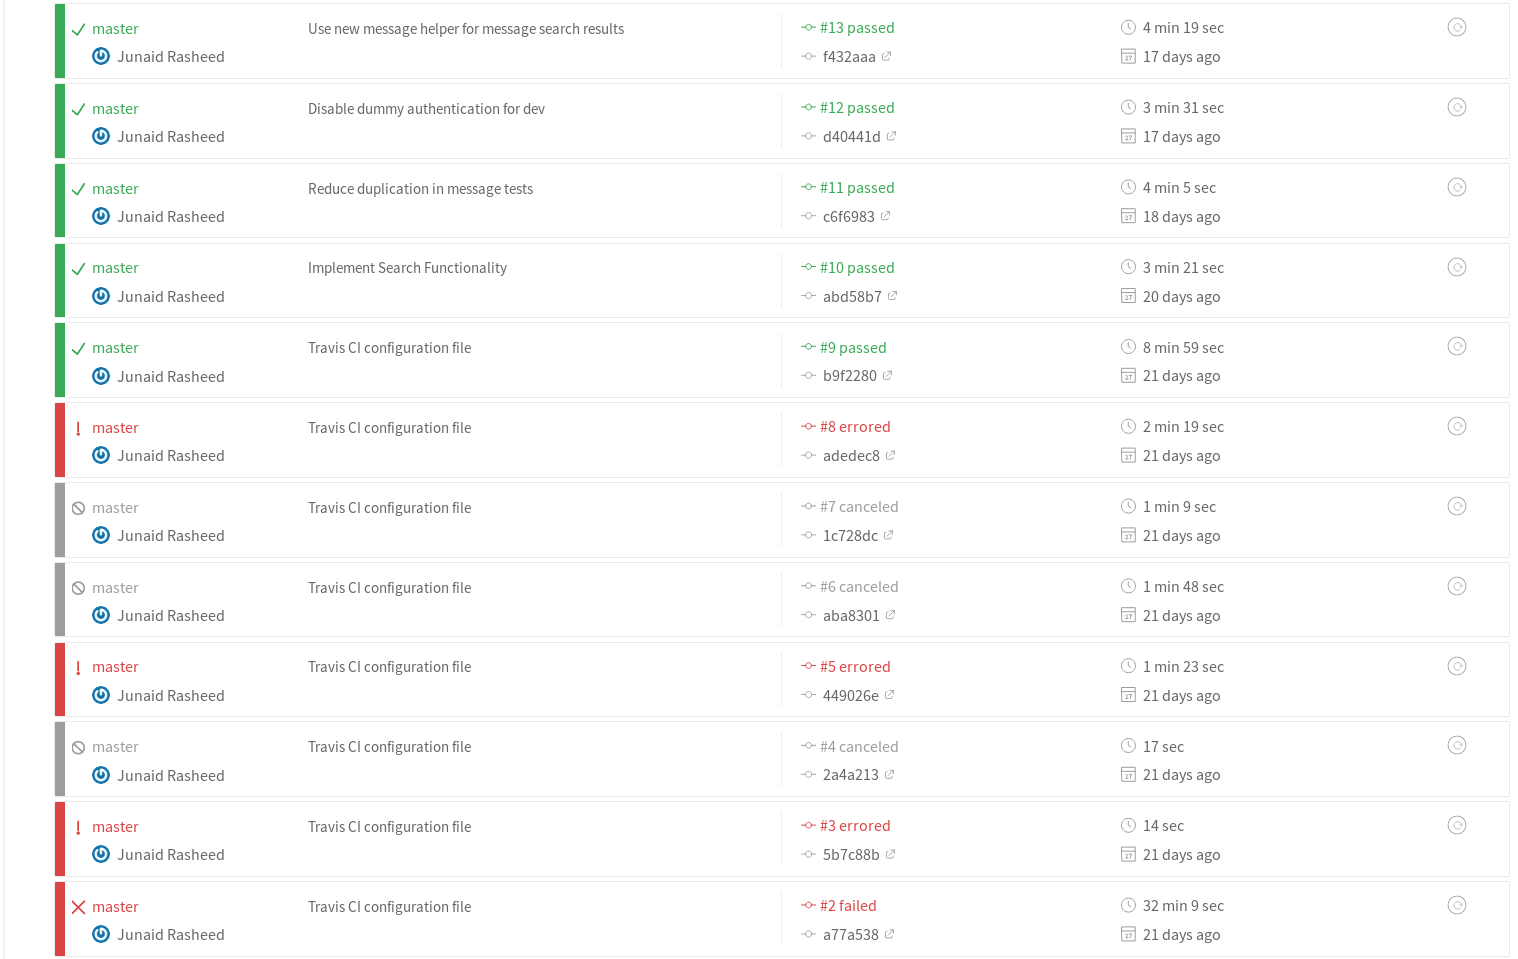
\includegraphics[width=0.9\textwidth]{final_report/pics/yesodTravis.png}
	\caption{Yesod Travis build times}
	\label{fig:yesodTravis}
\end{figure}

\begin{figure}[H]
	\centering
	
\includegraphics[width=0.9\textwidth]{final_report/pics/djangoTravis.png}
	\caption{Django Travis build times}
	\label{fig:djangoTravis}
\end{figure}

\section{Load Tests}

Load tests were ran using RedLine13 and Amazon EC2 servers. Load tests consisted of 80
users loading a specified page. Three tests were conducted. In one test, the home page
was loaded. In the two other tests, the profile page for a user who posted three
messages was loaded. Results can be found in ~\ref{tab:loadTests}

\begin{table}[H]
	\caption{Load Testing Page Load Speeds}
	\begin{center}
		\begin{tabular}{ | l | l | l |}
			\hline
			Page & Yesod (s) & Django (s) \\
			\hline
			Home & 4.96 & 5.54 \\
			Profile & 5.05 & 4.94 \\
			Profile & 4.97 & 5.13 \\
			Average & 4.99 & 5.20 \\
			\hline
		\end{tabular}
	\end{center}
	\label{tab:loadTest1}
\end{table}

\begin{table}[H]
	\caption{Load Testing Data Received}
	\begin{center}
		\begin{tabular}{ | l | l | l |}
			\hline
			Page & Yesod (MB) & Django (MB) \\
			\hline
			Home & 6.28 & 17.99 \\
			Profile & 6.76 & 18.74 \\
			Profile & 6.34 & 17.84 \\
			Average & 6.46 & 18.19 \\
			\hline
		\end{tabular}
	\end{center}
	\label{tab:dataTests}
\end{table}

\begin{figure}[H]
	\centering
	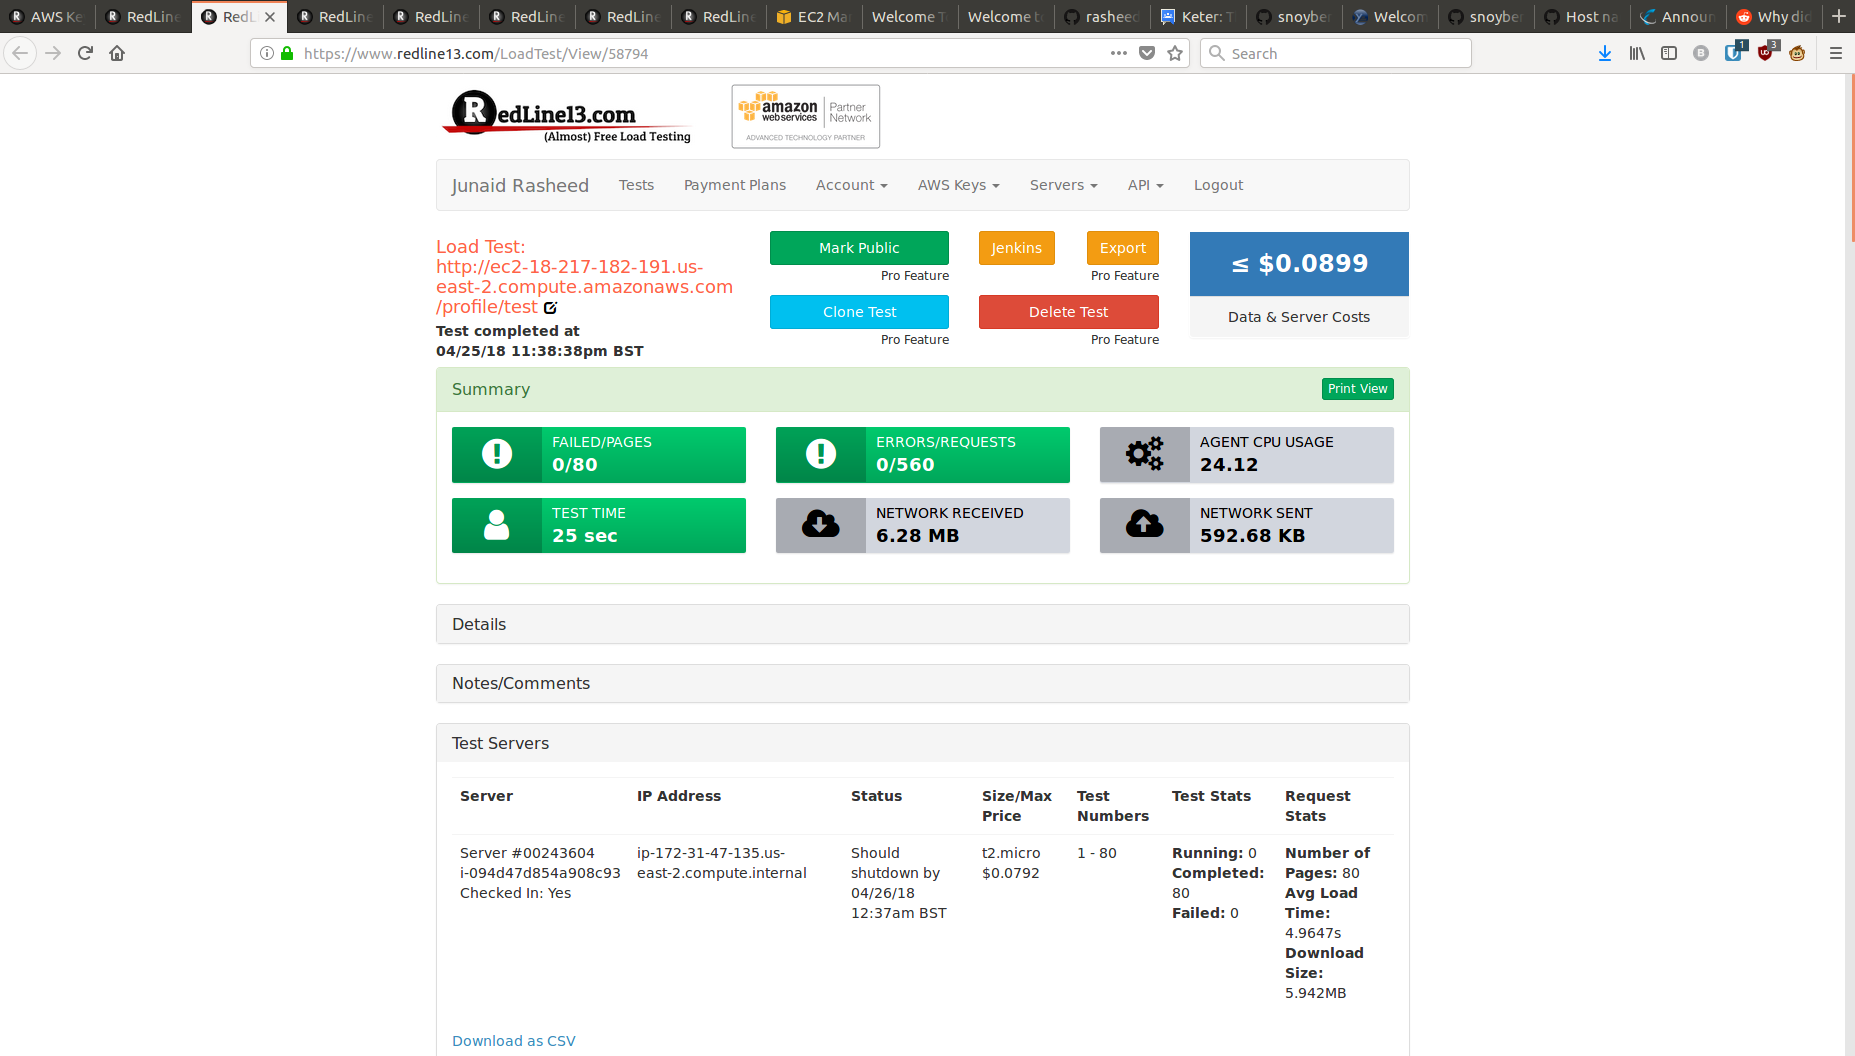
\includegraphics[width=0.9\textwidth]{final_report/pics/yesodLoadTest1.png}
	\caption{Yesod Load Test 1}
	\label{fig:yesodLoadTest1}
\end{figure}

\begin{figure}[H]
	\centering
	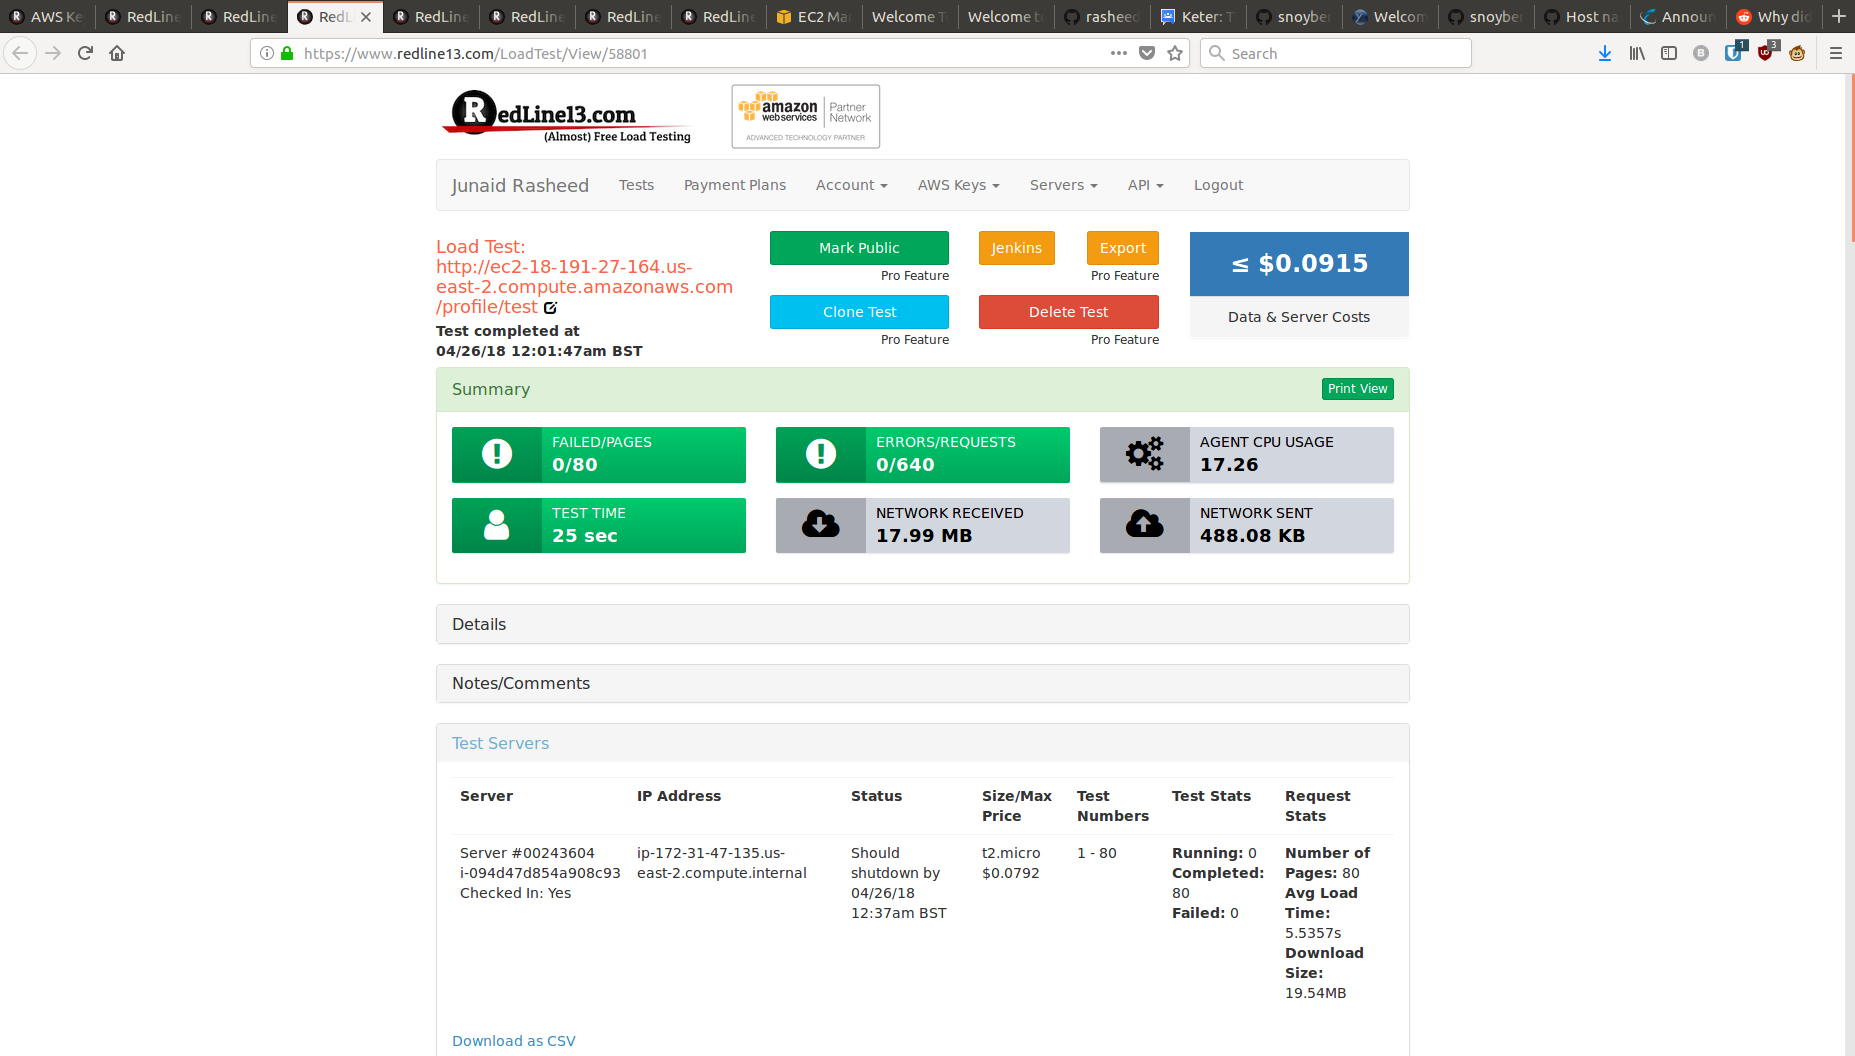
\includegraphics[width=0.9\textwidth]{final_report/pics/djangoLoadTest1.png}
	\caption{Django Load Test 1}
	\label{fig:djangoLoadTest1}
\end{figure}

\begin{figure}[H]
	\centering
	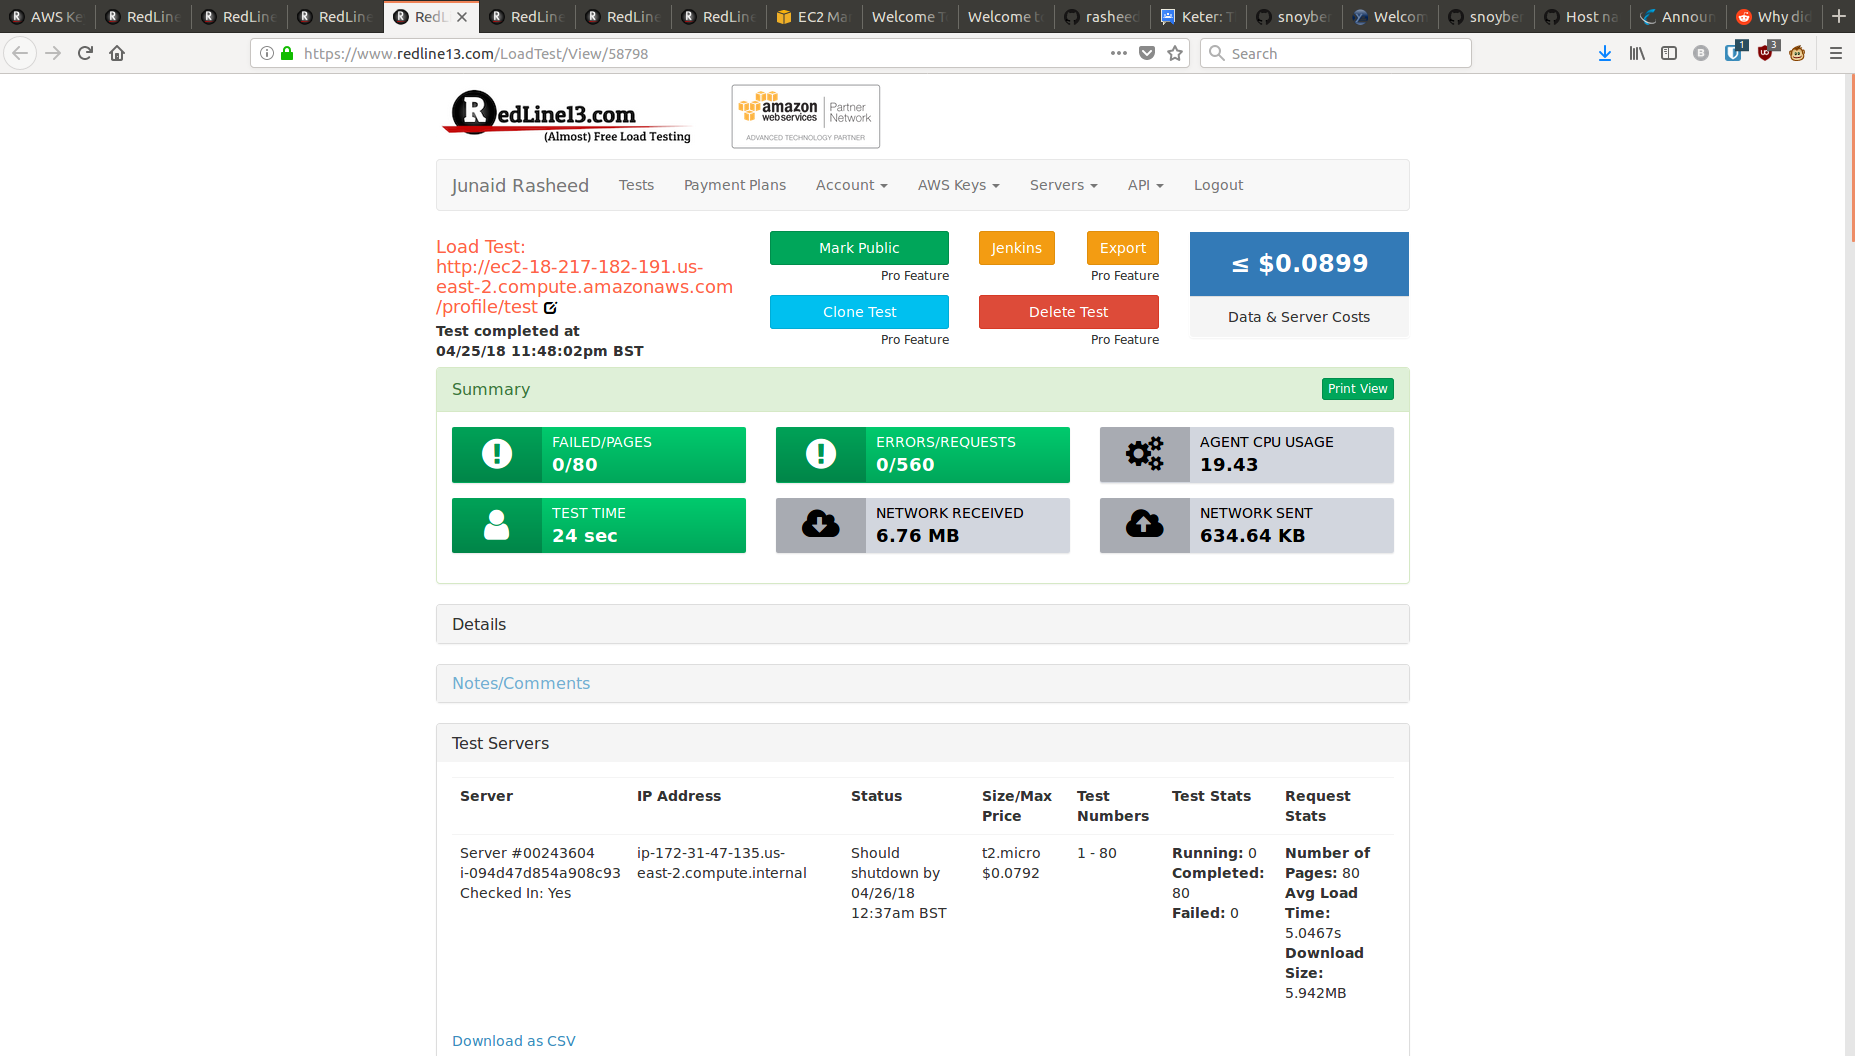
\includegraphics[width=0.9\textwidth]{final_report/pics/yesodLoadTest2.png}
	\caption{Yesod Load Test 2}
	\label{fig:yesodLoadTest2}
\end{figure}

\begin{figure}[H]
	\centering
	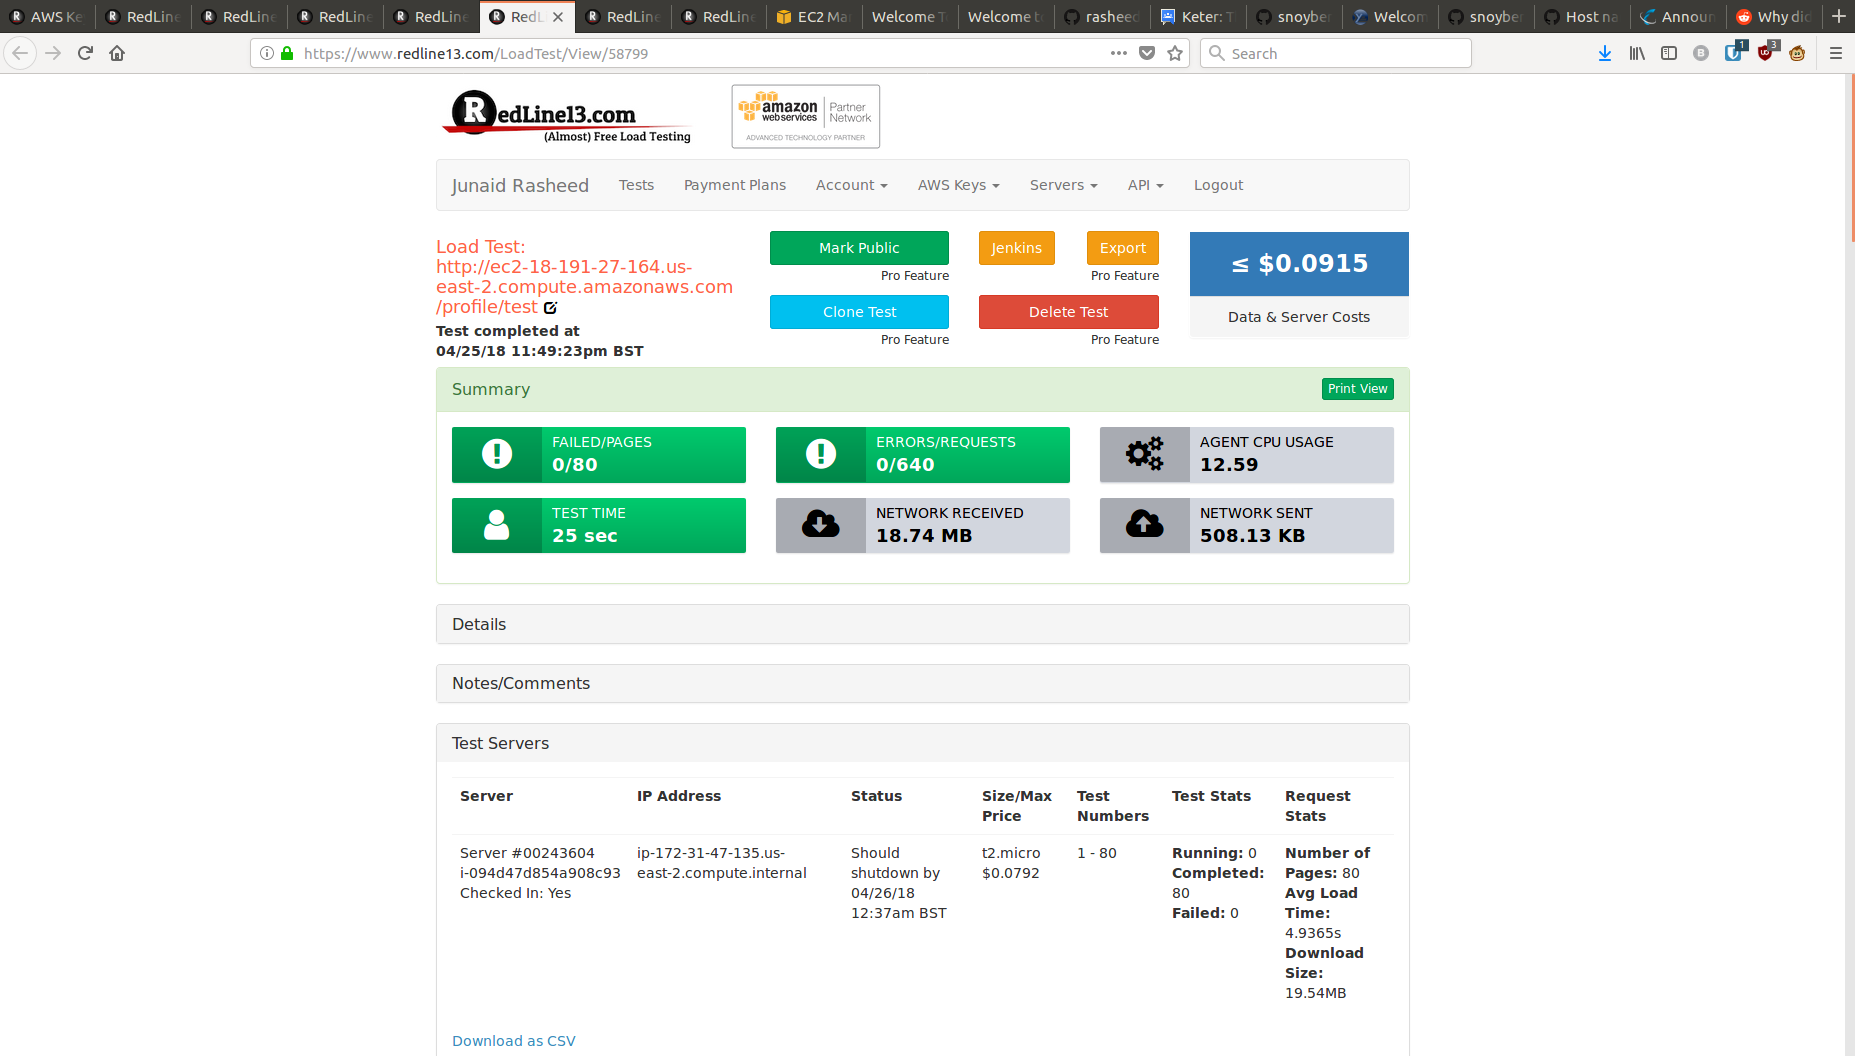
\includegraphics[width=0.9\textwidth]{final_report/pics/djangoLoadTest2.png}
	\caption{Django Load Test 2}
	\label{fig:djangoLoadTest2}
\end{figure}

\begin{figure}[H]
	\centering
	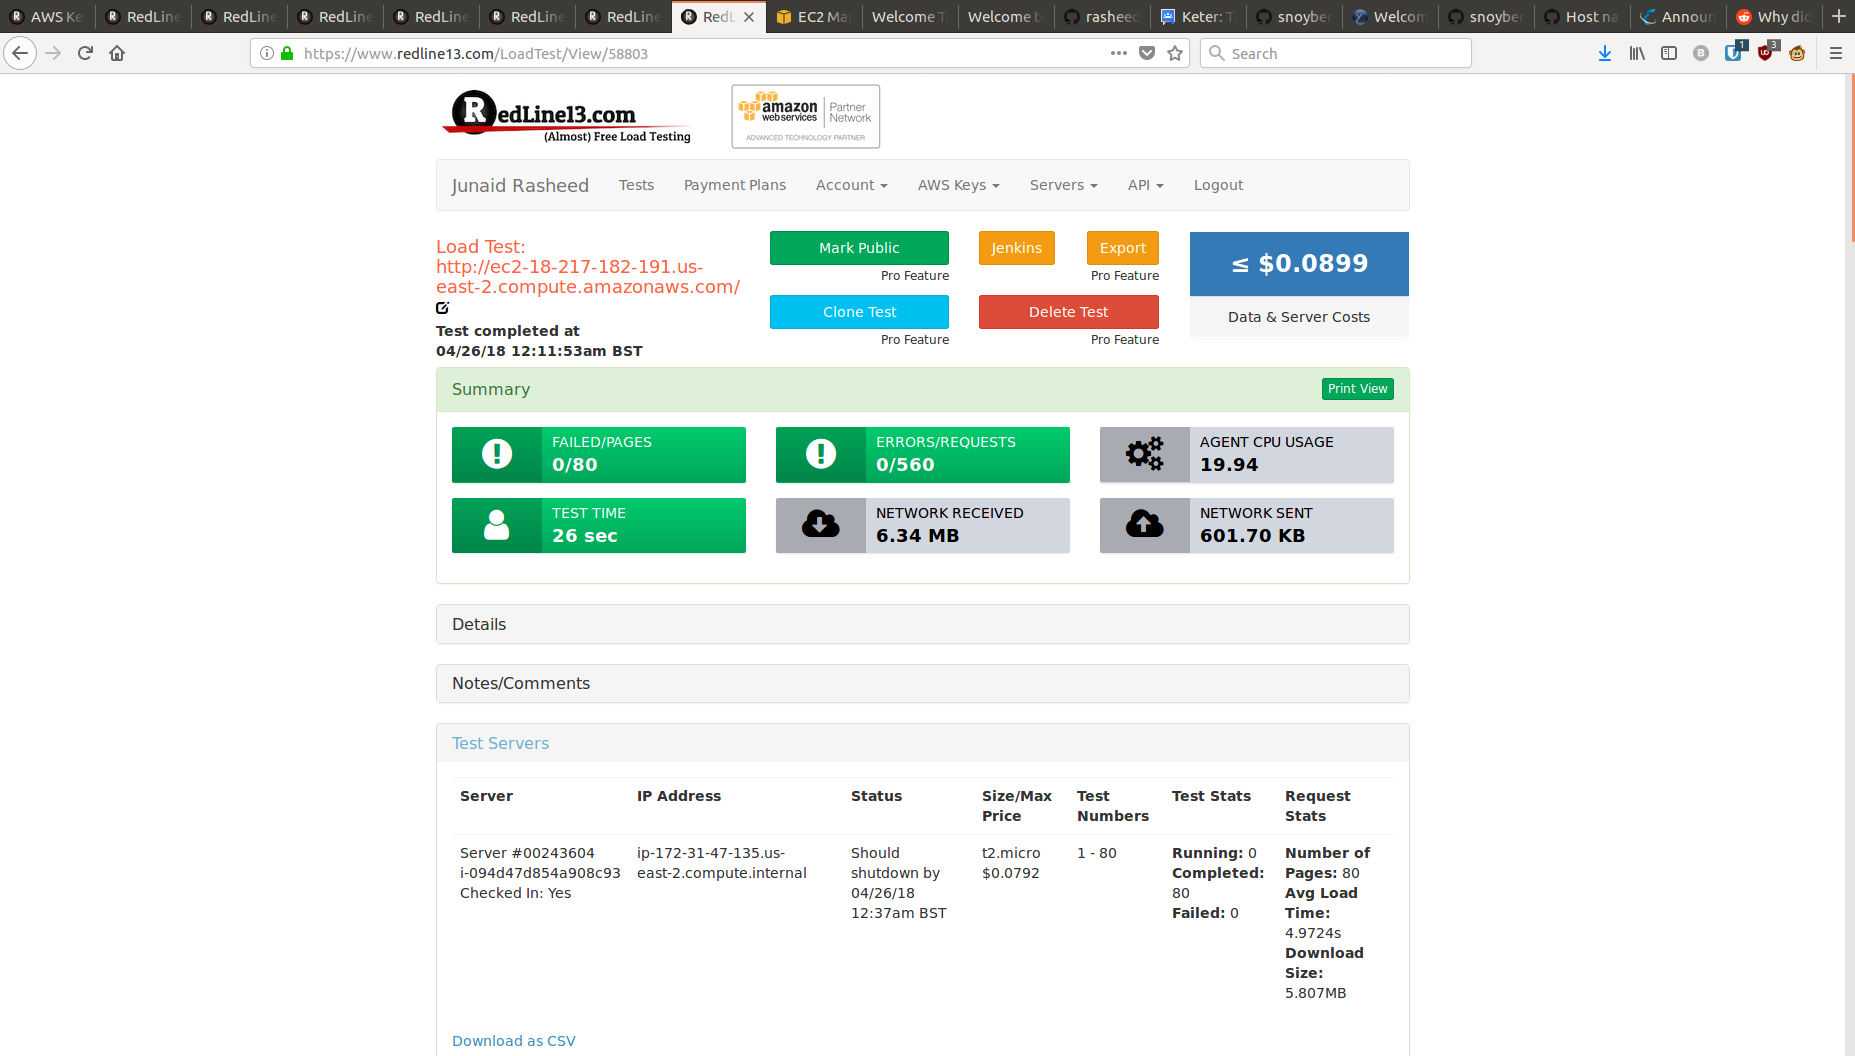
\includegraphics[width=0.9\textwidth]{final_report/pics/yesodLoadTest3.png}
	\caption{Yesod Load Test 3}
	\label{fig:yesodLoadTest3}
\end{figure}

\begin{figure}[H]
	\centering
	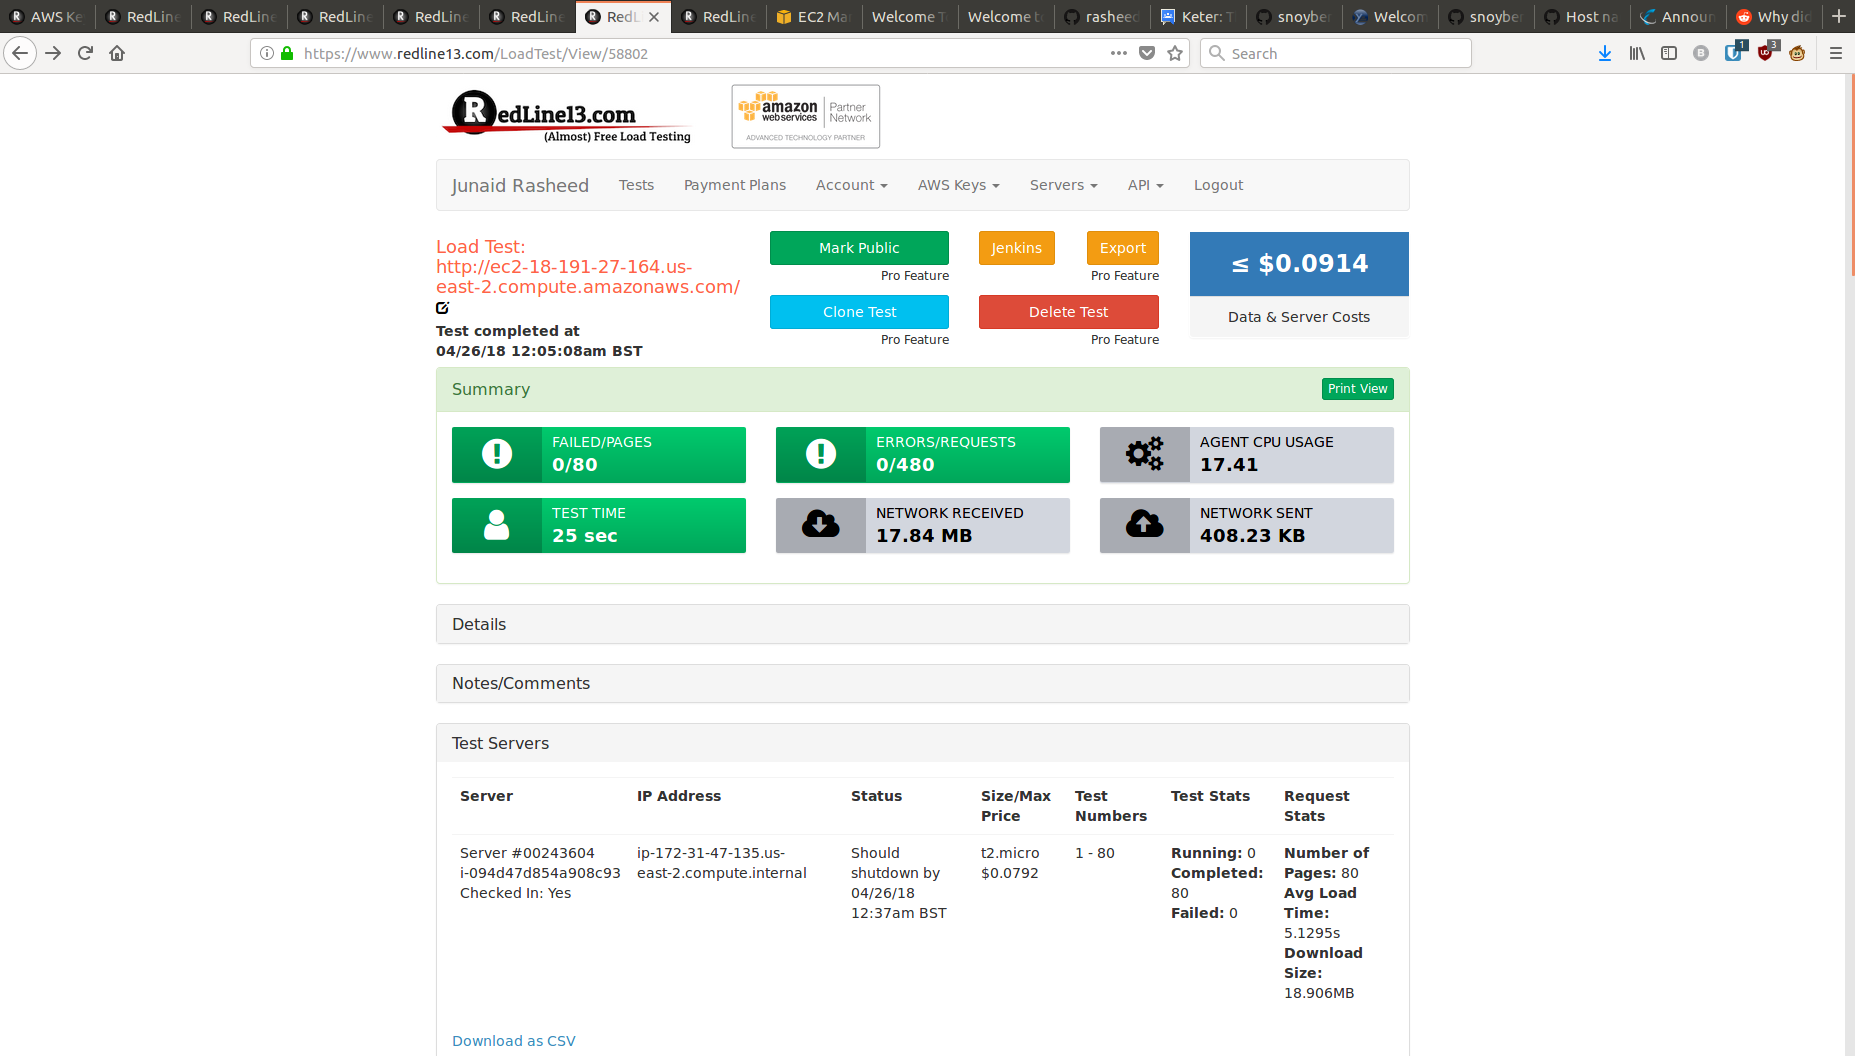
\includegraphics[width=0.9\textwidth]{final_report/pics/djangoLoadTest3.png}
	\caption{Django Load Test 3}
	\label{fig:djangoLoadTest3}
\end{figure}

\section{Introducing Realistic Errors}

For these tests, we purposefully made an error that could realistically happen.
After we made the error, we see the error messages that each framework gives us.

\subsection{Test 1}
When creating a message, try to save the form results rather than
the message extracted from the results into the database.

Yesod Results: Did not compile, unmatched type error. Tests can't be ran
as site did not compile.
Django Results: No error thrown even when submitting new message form.
Message not created. Database entry added, form data was converted to
string and added to Database. Tests passed because they were checking
the database count. This test was fixed to check the database content
as well.

\lstset{language={Haskell}}
\begin{lstlisting}[caption={Yesod Code Change},label={code:yesodTest1LC}]
	(Entity userId _) <- requireAuth
	((result, _), _) <- runFormPost $ messageForm userId
	case result of
		FormSuccess message -> do
			-- _ <- runDB . insert $ message -- original line 
			_ <- runDB . insert $ result -- new line 
\end{lstlisting}

\lstset{language={Python}}
\begin{lstlisting}[caption={Django Code Change},label={code:djangoTest1LC}]
	form = NewWireForm(request.POST)
	if form.is_valid():
		if request.user.is_authenticated:
			message = form.cleaned_data['message']
			try:
				# Message.objects.create(message_text=message, .. # original line
				Message.objects.create(message_text=form.cleaned_data, .. # changed line 1
				# Message.objects.create(message_text=form, .. # changed line 2, after previous line passed
\end{lstlisting}


\lstset{language={Haskell}}
\begin{lstlisting}[caption={Yesod Exception Message},label={code:yesodTest1Exception}]
	- Couldn't match type `PersistEntityBackend (FormResult Message)'
	with `SqlBackend'
	arising from a use of `insert'
	- In the second argument of `(.)', namely `insert'
	In the expression: runDB . insert
	In a stmt of a 'do' block: _ <- runDB . insert $ result
\end{lstlisting}

\begin{figure}[H]
	\centering
	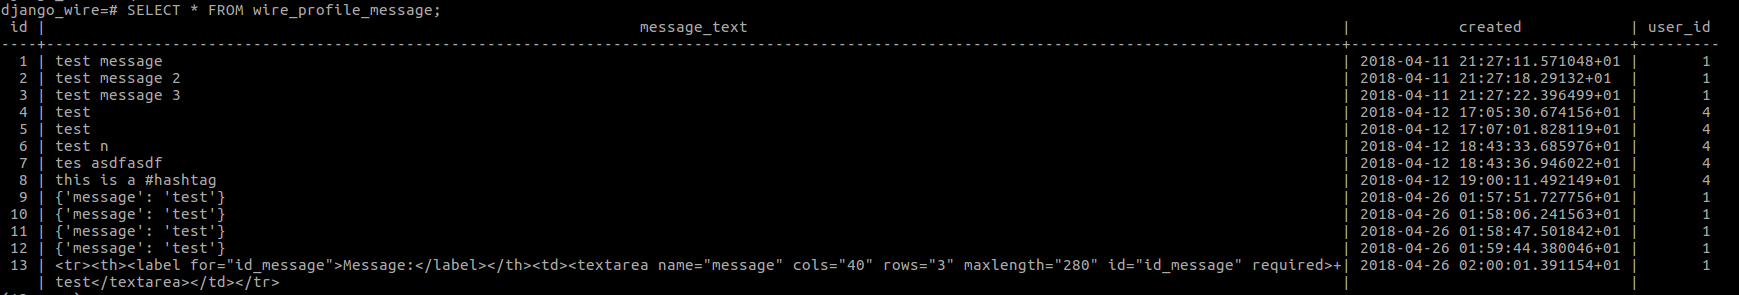
\includegraphics[width=0.9\textwidth]{final_report/pics/djangoMessageDB.png}
	\caption{Django Message Table Values}
	\label{fig:djangoMessageDBTest1}
\end{figure}

\subsection{Test 2}
Simply misspell a variable name. Most IDE tools catch this anyway but
error messages are useful to see. The misspelling was done in the code
that returns recommended users on the profile page. This code returns
data in JSON format.

Yesod: Did not compile, variable not in scope error. Compiler recommended
actual variable.

Django: AJAX request returned  a 500 error. Loading the page shows the
debug output. Exception thrown with message ``name `user' is not defined''.
Tests failed.

\lstset{language={Haskell}}
\begin{lstlisting}[caption={Yesod Code Change},label={code:yesodTest2LC}]
	Entity userId user <- requireAuth
	followers <- runDB $ selectList [FollowFollowerId ==. userId] []
	-- See: https://stackoverflow.com/questions/36727794/haskell-persistent-reusing-selectlist
	let followingIds = map (\(Entity _ (Follow _ followingId)) -> followingId) followers
	users <- runDB $ selectList [UserUsername !=. userUsername user, UserId /<-. followingIds] [LimitTo 5]
	let cleanUsers = map (\(Entity uid (User uname _ _)) -> (object ["id" .= uid, "username" .= uname])) users
	-- returnJson cleanUsers -- original line
	returnJson cleanUser -- new line
\end{lstlisting}

\lstset{language={Python}}
\begin{lstlisting}[caption={Django Code Change},label={code:djangoTest2LC}]
	if request.user.is_authenticated:
	follow_query = Follow.objects.filter(follower_id=request.user)
	users = User.objects.filter().exclude(id=request.user.id).exclude(username=excluded_username)\
		.exclude(followed_user__in=follow_query).values('username')[:5]
	# return JsonResponse(list(users), safe=False)  # original line
	return JsonResponse(list(user), safe=False)  # new line
\end{lstlisting}

\lstset{language={Haskell}}
\begin{lstlisting}[caption={Yesod Exception Message},label={code:yesodTest2Exception}]
	Variable not in scope: cleanUser
	Perhaps you meant `cleanUsers' (line 19)
\end{lstlisting}

\lstset{language={Python}}
\begin{lstlisting}[caption={Django Exception Message},label={code:djangoTest2Exception}]
	NameError at /get-recommended-users/test
	name `user' is not defined
\end{lstlisting}
